
\chapter{Transformée de Fourier du contour}

Les contours calculés sont codés avec le codage de Freeman.

\begin{figure}[h!]
    \centering
    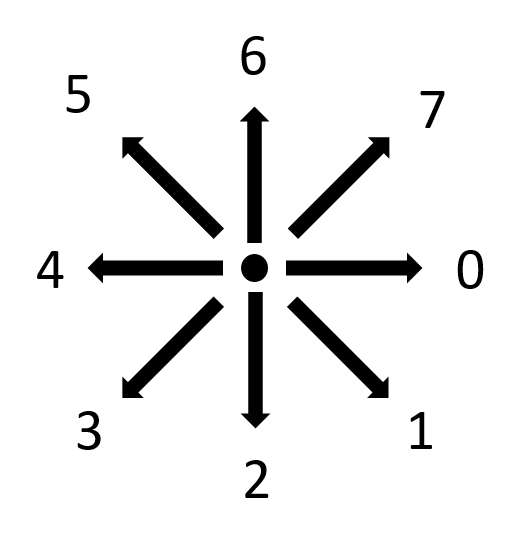
\includegraphics[scale=0.45]{assets/freeman-chain-encoding}
    \caption{Codage de Freeman d'une chaîne.}
	\label{fig:freeman-chain-encoding}
\end{figure}

On code un contour comme un $K$-uplet $a_1, \cdots a_K$ 
où les $a_i$ sont des entiers dans $\llbracket 0, 7 \rrbracket$. 
On notera $V = a_1 a_2 \cdots a_K$ la chaîne représentant le 
contour.

Cette chaîne définit un ensemble de points $(p_i)_i$ 
dont les coordonnées sont tous des entiers et vérifiant:
\[
\vecnorm{p_i - p_{i-1}} =
\begin{cases}
  1 \text{ si } a_i \text{ est paire;} \\
  \sqrt{2} \text{ sinon;} \\
\end{cases}
\]
avec $p_0 = (0,0)$.

On associe également, pour tout couple de points consécutifs 
un temps de traversé $\Delta t$ qui est égal à la distance 
séparant les deux points.
Cette quantité vérifie donc:
\[
\Delta t_i = 1 + \left( \frac{\sqrt(2) - 1}{2} \right) \left( 1 - (-1)^{a_i} \right)
\]

Le temps mis pour traverser les $p$ premiers liens de la chaîne vaut donc 
\[
t_p = \sum_{i = 1}^{p} \Delta t_i
\]
et la période de la chaîne est $T = t_K$.



Considérons que notre contour est une fonction périodique de 
période $T$ de $\mathbb{R}$ dans $\mathbb{R}^2$ dont les composantes 
sont $x(t)$ et $y(t)$.
Alors sa décomposition en séries de Fourier s'écrit
\[
x(t) = A_0 + \sum_{n = 1}^{+\infty} a_n \cos\left(\frac{2n\pi t}{T}\right) 
  + b_n \sin\left(\frac{2n\pi t}{T}\right) 
\]
où
\[
A_0 = \frac{1}{T} \int_{0}^{T} x(t) \mathrm{d}t  \qquad
a_n = \frac{2}{T} \int_{0}^{T} x(t) \cos\left(\frac{2n\pi t}{T}\right)  \mathrm{d}t  \qquad
b_n = \frac{2}{T} \int_{0}^{T} x(t) \sin\left(\frac{2n\pi t}{T}\right)  \mathrm{d}t 
\]

Nous allons calculer ces coefficients de manière explicite en écrivant 
la dérivée $x'(t)$ de deux manières.
On rappelle que $x$ est dérivable en tout point $t \in ]0, T[$ 
n'appartenant pas à $\{ t_1, \cdots, t_K \}$.

La première écriture s'obtient en appliquant une transformée de Fourier 
à $x'$ qui est une fonction périodique de période $T$. 
\[
x'(t) = \sum_{n = 1}^{+\infty} \alpha_n \cos\left(\frac{2n\pi t}{T}\right) 
  + \beta_n \sin\left(\frac{2n\pi t}{T}\right) 
\]
où
\[
\alpha_n = \frac{2}{T} \int_{0}^{T} x'(t) \cos\left(\frac{2n\pi t}{T}\right)  \mathrm{d}t  \qquad \qquad
\beta_n = \frac{2}{T} \int_{0}^{T} x'(t) \sin\left(\frac{2n\pi t}{T}\right)  \mathrm{d}t 
\]
Il n'y a évidemment pas de terme constant dans cette écriture car 
l'intégrale de $x'$ sur une période vaut 0 puisque $x(0) = x(T)$.

Ces quantités sont faciles à calculer car $x'$ est constante par 
morceaux.
\[
x'(t) = \frac{\Delta x_p}{\Delta t_p} \text{ pour } t_{p-1} < t < t_p
\]

On obtient donc
\begin{align*}
\alpha_n &= \frac{2}{T} \sum_{p = 1}^{K} \frac{\Delta x_p}{\Delta t_p} \int_{t_{p-1}}^{t_p} \cos\left(\frac{2n\pi t}{T}\right)  \mathrm{d}t  \\
         &= \frac{1}{n \pi} \sum_{p = 1}^{K} \frac{\Delta x_p}{\Delta t_p} \left( \sin\left(\frac{2n\pi t_p}{T}\right) - \sin\left(\frac{2n\pi t_{p-1}}{T}\right)  \right)
\end{align*}
De même, 
\[
\beta_n = -\frac{1}{n \pi} \sum_{p = 1}^{K} \frac{\Delta x_p}{\Delta t_p} \left( \cos\left(\frac{2n\pi t_p}{T}\right) - \cos\left(\frac{2n\pi t_{p-1}}{T}\right)  \right)
\]

La seconde expression de $x'(t)$ est obtenue en dérivant directement son 
expression sous forme de série.
\[
x'(t) = \frac{2n\pi}{T}\sum_{n = 1}^{+\infty} -a_n \sin\left(\frac{2n\pi t}{T}\right) 
  + b_n \cos\left(\frac{2n\pi t}{T}\right) 
\]

On écrit ensuite l'égalité des coefficients devant les sinus et cosinus 
d'une période donnée.
\[
\begin{cases}
  \alpha_n = \frac{2n\pi}{T} b_n \\
  \beta_n = \frac{2n\pi}{T} a_n
\end{cases}
\]
Au final, 
\[
a_n = \frac{T}{2 n^2 \pi^2} \sum_{p = 1}^{K} \frac{\Delta x_p}{\Delta t_p} \left[ \cos\left(\frac{2n\pi t_p}{T}\right) - \cos\left(\frac{2n\pi t_{p-1}}{T}\right) \right]
\]
\[
b_n = \frac{T}{2 n^2 \pi^2} \sum_{p = 1}^{K} \frac{\Delta x_p}{\Delta t_p} \left[ \sin\left(\frac{2n\pi t_p}{T}\right) - \sin\left(\frac{2n\pi t_{p-1}}{T}\right) \right]
\]

On peut appliquer le même raisonnement pour $y(t)$ et on obtiendra des 
coefficients $C_0$, $c_n$ et $d_n$ vérifiant les mêmes équations.

On pourra utiliser les coefficients $a_n, b_n, c_n, d_n$ comme features.
